\documentclass{beamer}
\usetheme{Singapore}
\usepackage{changepage}

%\usepackage{pstricks,pst-node,pst-tree}
\usepackage{amssymb,latexsym}
\usepackage{tikz}
\usepackage{graphicx}
\usepackage{fancyvrb}
\usepackage{hyperref}
\usepackage{fancybox}
\usepackage[listings]{tcolorbox}

\definecolor{codegreen}{rgb}{0,0.6,0}
\definecolor{codegray}{rgb}{0.5,0.5,0.5}
\definecolor{codepurple}{rgb}{0.58,0,0.82}
\definecolor{backcolour}{rgb}{0.95,0.95,0.92}

\lstdefinestyle{mystyle}{
    language=Python,
    backgroundcolor=\color{backcolour},   
    commentstyle=\color{codegreen},
    keywordstyle=\color{magenta},
    numberstyle=\tiny\color{codegray},
    stringstyle=\color{codepurple},
    basicstyle=\ttfamily\footnotesize,
    breakatwhitespace=false,         
    breaklines=true,                 
    captionpos=b,                    
    keepspaces=true,                 
    numbers=left,                    
    numbersep=5pt,                  
    showspaces=false,                
    showstringspaces=false,
    showtabs=false,                  
    tabsize=2,
    escapechar=|,
    frame=single
}

\lstset{style=mystyle}


\newcommand{\bi}{\begin{itemize}}
\newcommand{\li}{\item}
\newcommand{\ei}{\end{itemize}}
\newcommand{\Show}[1]{
\begin{center}
\shadowbox{\begin{minipage}{0.8\textwidth}
          #1
          \end{minipage}}
\end{center}
}
\newcommand{\arrow}{\ensuremath{\rightarrow}}

\newcommand{\uparr}{\ensuremath{\uparrow}}


\newcommand{\fig}[2]{\centerline{\includegraphics[width=#1\textwidth]{#2}}}

\newcommand{\bfr}[1]{\begin{frame}[fragile]\frametitle{{ #1 }}}
\newcommand{\efr}{\end{frame}}

\newcommand{\cola}{\begin{columns}\begin{column}{0.5\textwidth}}
\newcommand{\colb}{\end{column}\begin{column}{0.5\textwidth}}
\newcommand{\colc}{\end{column}\end{columns}}


\title{Think Python 2e, Chapter 11 Notes}
\author{Dictionaries}

\begin{document}

\begin{frame}
\maketitle
\end{frame}

\bfr{A dictionary is a \bf mapping}

\cola
\begin{tabular}{|r|l|}\hline
{\bf English} & {\bf Spanish} \\ \hline
one & uno \\
two & dos \\
three & tres \\
cat & gato \\
dog & perro \\
priest & sacerdote \\
... & ... \\\hline
\end{tabular}
\colb
\fbox{\bf English} \ensuremath{\longrightarrow} \fbox{\bf Spanish}

\colc

\end{frame}


\bfr{Dictionaries in python}
\begin{lstlisting}
>>> eng2sp = dict()
>>> eng2sp
{}
>>> eng2sp['one'] = 'uno'
>>> eng2sp
{'one': 'uno'}
\end{lstlisting}
The output format is also an input format:
\begin{lstlisting}
>>> eng2sp ={'one':'uno', 'two':'dos', 'three':'tres'}
>>> eng2sp
{'one': 'uno', 'three': 'tres', 'two': 'dos'}
\end{lstlisting}
Note that the order of items is random.

\end{frame}


\bfr{Accessing dictionaries in python}
\begin{lstlisting}
>>> eng2sp['two']
'dos'
>>> eng2sp['four']
KeyError: 'four'
>>> len(eng2sp)
3
>>> 'one' in eng2sp
True
>>> 'uno' in eng2sp
False
>>> vals = eng2sp.values()
>>> 'uno' in vals
True
\end{lstlisting}

\end{frame}

\bfr{Histograms with dictionaries}

\begin{lstlisting}
def histogram(s):
    d = dict()
    for c in s:
        if c not in d:
            d[c] = 1
        else:
            d[c] += 1
    return d
\end{lstlisting}
\begin{lstlisting}
>>> h = histogram('brontosaurus')
>>> h
{'a': 1, 'b': 1, 'o': 2, 'n': 1, 's': 2, 'r': 2, 'u': 2, 't': 1}
\end{lstlisting}

See my histogram of {\em Moby Dick}

\end{frame}
\bfr{Looping with dictionaries}

\begin{lstlisting}
def print_hist(h):
    for c in h:
        print(c, h[c])
\end{lstlisting}
\begin{lstlisting}
>>> h = histogram('parrot')
>>> print_hist(h)
a 1
p 1
r 2
t 1
o 1
\end{lstlisting}
\begin{lstlisting}
>>> for key in sorted(h):
...     print(key, h[key])
a 1
o 1
p 1
r 2
t 1
\end{lstlisting}
\end{frame}

\bfr{Reverse lookup}

\begin{lstlisting}
def reverse_lookup(d, v):
    for k in d:
        if d[k] == v:
            return k
    raise LookupError()
\end{lstlisting}
\begin{lstlisting}
>>> h = histogram('parrot')
>>> key = reverse_lookup(h, 2)
>>> key
'r'
\end{lstlisting}
\begin{lstlisting}
>>> key = reverse_lookup(h, 3)
Traceback (most recent call last):
  File "<stdin>", line 1, in <module>
  File "<stdin>", line 5, in reverse_lookup
LookupError
\end{lstlisting}
\end{frame}
\bfr{Raise with message}
\begin{lstlisting}
>>> raise LookupError('value does not appear in the dictionary')
Traceback (most recent call last):
  File "<stdin>", line 1, in ?
LookupError: value does not appear in the dictionary

\end{lstlisting}

\end{frame}

\bfr{Invert a dictionary}

\begin{lstlisting}
def invert_dict(d):
    inverse = dict()
    for key in d:
        val = d[key]
        if val not in inverse:
            inverse[val] = [key]
        else:
            inverse[val].append(key)
    return inverse
\end{lstlisting}

\end{frame}

\bfr{Invert example}

\begin{lstlisting}
>>> hist = histogram('parrot')
>>> hist
{'a': 1, 'p': 1, 'r': 2, 't': 1, 'o': 1}
>>> inverse = invert_dict(hist)
>>> inverse
{1: ['a', 'p', 't', 'o'], 2: ['r']}
\end{lstlisting}

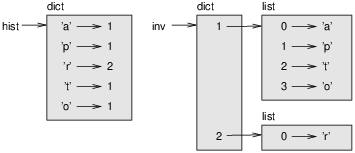
\includegraphics{statediagram11-1}

\end{frame}

\bfr{Lists cannot be keys}

\begin{lstlisting}
>>> t = [1, 2, 3]
>>> d = dict()
>>> d[t] = 'oops'
Traceback (most recent call last):
  File "<stdin>", line 1, in ?
TypeError: list objects are unhashable

\end{lstlisting}



\end{frame}

\bfr{Keys and hashing}
\bi
\li Dictionaries are implemented using {\bf hashtables}
\li A {\bf hash} is a function that takes a value and returns an integer.
\li Dictionaries use hashes of the keys as indexes.
\li This only works if keys are immutable.
\li If a key were mutable, the hashtable would have to change every time the key changed.
\li Lists are mutable, so cannot be keys.
\li Dictionaries are mutable, so cannot be keys.
\li Both lists and dictionaries can be values.
\ei

\end{frame}

\bfr{Redundant work in naive implementations}

\begin{lstlisting}
def fibonacci(n):
    if n < 2:
        return n
    else:
        return fibonacci(n-1) + fibonacci(n-2)
\end{lstlisting}
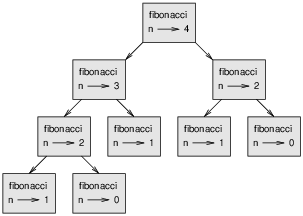
\includegraphics{callgraph11-2}


\end{frame}

\bfr{Memoizing}

\begin{lstlisting}
known = {0:0, 1:1}

def fibonacci(n):
    if n in known:
        return known[n]

    res = fibonacci(n-1) + fibonacci(n-2)
    known[n] = res
    return res
\end{lstlisting}
\pause
Uses global variable.

We'll see later how to get rid of that.
\end{frame}

\bfr{Global variables}
\cola
\begin{lstlisting}
x = 10
def show_global():
    print(x)
show_global()
print(x)
def mod_global_bad():
    x = 20
    print(x)
mod_global_bad()
print(x)
def mod_global_good():
    global x
    x = 20
    print(x)
mod_global_good()
print(x)
\end{lstlisting}
\colb
\begin{lstlisting}
10
10
20
10
20
20
\end{lstlisting}
\colc
\end{frame}

\bfr{Good use of global variables}
\begin{lstlisting}
verbose = True

def example1():
    if verbose:
        print('Running example1')
\end{lstlisting}
\end{frame}

\bfr{What's wrong with this example?}
\begin{lstlisting}
been_called = False

def example2():
    been_called = True         # WRONG
\end{lstlisting}
\end{frame}

\bfr{What's wrong with this example?}
\begin{lstlisting}
count = 0

def example3():
    count = count + 1          # WRONG
\end{lstlisting}
\end{frame}


\bfr{Global mutable objects can be mutated locally}
\begin{lstlisting}
known = {0:0, 1:1}

def example4():
    known[2] = 1
\end{lstlisting}
\end{frame}

\bfr{Globals}
\bi
\li Can be confusing
\li Declare them in functions with \lstinline{global}
\li Avoid using them
\ei

\end{frame}

\bfr{Debugging}
\bi
\li Scale down the input.
\li Check summaries of outputs.
\li Check types of outputs
\li Write sanity checks:
\bi\li averages should not be larger than maximum
\li averages should not be smaller than the minimum
\ei
\li Write consistency checks
\bi\li Number of sentences $<$ number of words
\ei
\li Format the output so it's easy to spot errors
\bi\li check out \lstinline{pprint}
\ei
\ei

\end{frame}

\bfr{Vocabulary}
\begin{description}

\li[mapping:]
A relationship in which each element of one set corresponds to an element of another set.
\li[dictionary:]
A mapping from keys to their corresponding values.
\li[key-value pair:]
The representation of the mapping from a key to a value.
\li[item:]
In a dictionary, another name for a key-value pair.
\li[key:]
An object that appears in a dictionary as the first part of a key-value pair.
\li[value:]
An object that appears in a dictionary as the second part of a key-value pair. This is more specific than our previous use of the word “value”.
\end{description}
\end{frame}
\bfr{Vocabulary}
\begin{description}
\li[implementation:]
A way of performing a computation.
\li[hashtable:]
The algorithm used to implement Python dictionaries.
\li[hash function:]
A function used by a hashtable to compute the location for a key.
\li[hashable:]
A type that has a hash function. Immutable types like integers, floats and strings are hashable; mutable types like lists and dictionaries are not.
\li[lookup:]
A dictionary operation that takes a key and finds the corresponding value.
\li[reverse lookup:]
A dictionary operation that takes a value and finds one or more keys that map to it.
\end{description}
\end{frame}
\bfr{Vocabulary}
\begin{description}
\li[raise statement:]
A statement that (deliberately) raises an exception.
\li[singleton:]
A list (or other sequence) with a single element.
\li[call graph:]
A diagram that shows every frame created during the execution of a program, with an arrow from each caller to each callee.
\li[memo:]
A computed value stored to avoid unnecessary future computation.
\end{description}
\end{frame}
\bfr{Vocabulary}
\begin{description}
\li[global variable:]
A variable defined outside a function. Global variables can be accessed from any function.
\li[global statement:]
A statement that declares a variable name global.
\li[flag:]
A boolean variable used to indicate whether a condition is true.
\li[declaration:]
A statement like global that tells the interpreter something about a variable.
\end{description}
\end{frame}


\end{document}
